\let\negmedspace\undefined
\let\negthickspace\undefined
\documentclass[journal]{IEEEtran}
\usepackage[a5paper, margin=10mm, onecolumn]{geometry}
%\usepackage{lmodern} % Ensure lmodern is loaded for pdflatex
\usepackage{tfrupee} % Include tfrupee package

\setlength{\headheight}{1cm} % Set the height of the header box
\setlength{\headsep}{0mm}     % Set the distance between the header box and the top of the text

\usepackage{gvv-book}
\usepackage{gvv}
\usepackage{cite}
\usepackage{amsmath,amssymb,amsfonts,amsthm}
\usepackage{algorithmic}
\usepackage{graphicx}
\usepackage{textcomp}
\usepackage{xcolor}
\usepackage{txfonts}
\usepackage{listings}
\usepackage{enumitem}
\usepackage{mathtools}
\usepackage{gensymb}
\usepackage{comment}
\usepackage[breaklinks=true]{hyperref}
\usepackage{tkz-euclide} 
\usepackage{listings}
% \usepackage{gvv}                                        
\def\inputGnumericTable{}                                 
\usepackage[latin1]{inputenc}                                
\usepackage{color}                                            
\usepackage{array}                                            
\usepackage{longtable}                                       
\usepackage{calc}                                             
\usepackage{multirow}                                         
\usepackage{hhline}                                           
\usepackage{ifthen}                                           
\usepackage{lscape}
\begin{document}

\bibliographystyle{IEEEtran}
\vspace{3cm}

\title{7.4.18}
\author{EE25BTECH11011 - Navya}
% \maketitle
% \newpage
% \bigskip
{\let\newpage\relax\maketitle}

\renewcommand{\thefigure}{\theenumi}
\renewcommand{\thetable}{\theenumi}
\setlength{\intextsep}{10pt} % Space between text and floats
\textbf{Question}:\\
If the lines $3x-4y-7=0$ and $2x-3y-5=0$ are two diameters of a circle of area $49\pi$ square units, find the equation of the circle.

\begin{enumerate}
  \item $x^2+y^2+2x-2y-47=0$
  \item $x^2+y^2+2x-2y-62=0$
  \item $x^2+y^2-2x+2y-62=0$
  \item $x^2+y^2-2x+2y-47=0$
\end{enumerate}

\textbf{Solution:}

The general equation of a circle can be written as
\begin{align}
\mathbf{x}^T \mathbf{x} + 2 \mathbf{b}^T \mathbf{x} + c = 0,
\end{align}
where
\begin{align}
\mathbf{x} = \begin{bmatrix} x \\ y \end{bmatrix}, \quad
\mathbf{b} = \begin{bmatrix} b_1 \\ b_2 \end{bmatrix}, \quad
c \in \mathbb{R}.
\end{align}

The center $\mathbf{c}$ and radius $r$ relate to $\mathbf{b}$ and $c$ as:
\begin{align}
\mathbf{c} &= -\mathbf{b}, \\
r &= \sqrt{\mathbf{b}^T \mathbf{b} - c}.
\end{align}

Since the lines are diameters, the center lies on both:
\begin{align}
\mathbf{n}_1^T \mathbf{c} &= d_1, \\
\mathbf{n}_2^T \mathbf{c} &= d_2,
\end{align}
where
\begin{align}
\mathbf{n}_1 = \begin{bmatrix} 3 \\ -4 \end{bmatrix}, \quad d_1 = 7, \quad
\mathbf{n}_2 = \begin{bmatrix} 2 \\ -3 \end{bmatrix}, \quad d_2 = 5.
\end{align}


In matrix form,
\begin{align}
\begin{bmatrix}
3 & -4 \\
2 & -3
\end{bmatrix}
\mathbf{c} =
\begin{bmatrix}
7 \\
5
\end{bmatrix}.
\end{align}

Solving for $\mathbf{c}$:
\begin{align}
\mathbf{c} =
\begin{bmatrix}
1 \\
-1
\end{bmatrix}.
\end{align}

The area of the circle is $49\pi$, so radius is
\begin{align}
r = 7
\end{align}

and from the radius relation,
\begin{align}
r^2 &= \mathbf{c}^T \mathbf{c} - c, \\
49 &= 1^2 + (-1)^2 - c = 2 - c, \\
\implies c &= 2 - 49 = -47.
\end{align}

so the equation is
\begin{align}
\mathbf{x}^T \mathbf{x} + 2 \mathbf{b}^T \mathbf{x} + c = 0,
\end{align}
which expands to
\begin{align}
x^2 + y^2 + 2(-1)x + 2(1)y - 47 = 0,
\end{align}
Therefore, the equation of the circle is
 \begin{align}
\boxed{x^2 + y^2 - 2x + 2y - 47 = 0.}
 \end{align}

\begin{figure}[h!]
    \centering
    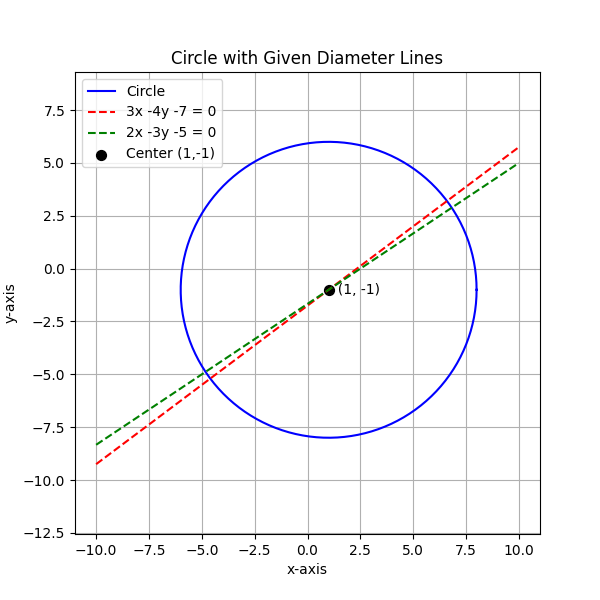
\includegraphics[width=0.6\textwidth]{figs/fig13.png}
    \label{fig:division}
\end{figure}
\end{document}